
\chapter{The A of ABC of Indian chronology*: Dimensions of the Aryan problem revisited in 2017}

\Authorline{Manogna Sastry \& Megh Kalyanasundaram}

*In reference to the authors’ framework seen in earlier Swadeshi Indology work

\section{Introduction}

From Indomania to Indophobia\index{Indophobia}, Europe’s appraisal of India has seen ebb and flow in a manner that has changed the course of both continents for several centuries. While numerous ancient Greeks, Romans and Arabs as well as Germans and French heaped abundantly generous and insightful praise about the character of the Indian culture in the early centuries of contact, the advent of colonization changed the tide. The initial waves of positive wonder and awe turned into a systematic destruction of everything the Indian held as formative and precious, be it religion or scientific achievements or even the very character of the Indian, using the faithful colonial tools of malicious and insidious criticism from a well-developed kit of propaganda, thusly painting a highly revolting portrait of the ancient land and consequently providing legitimacy to the act of looting an entire people for centuries. Indeed, the speed with which the narrative accorded to India by Britain was revamped beyond recognition—from hailing it as among the greatest civilizations to one which needed to be saved and transformed according to the sagely wisdom of the colonizer—openly betrays the nefarious intentions of the oppressor.

Among the most potent tools in the British propaganda kit was the role played by its intelligentsia. In the garb of studying Indian culture, the colonial academia did a phenomenally thorough job of systematically dismantling every aspect of Indian culture and infiltrating it with Christian evangelist anthems. Disfiguring the very spine of Indian culture began with attacking all aspects of the \textit{sanātana dharma}. Today, the indentation that ancient India had no sense of historical thinking has become a maxim and it is to the colonizer that the Indian owes gratitude for this very generous appraisal. The British went further from this imperious proclamation to give more of their largesse—a revised historical account and new theories of the very origin of the land’s culture. And at the heart of this peremptory legacy lies a revised chronology that was constructed of Indian history, which successfully enabled the colonizer in his designs.


\section{“Aryan” problem in 2017: Western\hfill \break academia to Indian politics - some\hfill \break manifestations}

It is to the work of several pioneers of western Indology that the most critical conceptions of colonization are credited - the common structure of Greek, Latin, German, Persian and Sanskrit as well as the apparent common origin of Sanskrit and European languages to a Proto-Indo-European (PIE) language and its corresponding homeland. The association of race, with the new European conception of a PIE language, by Indologists such as Max Muller\index{Max Muller} and Adolphe Pictet, marks one of the most crucial milestones that set the ball rolling on some disastrously consequential fallacies for India. \textit{Ārya},\index{Arya@Ārya} from being a term that was used to denote a highly cultured person, became Aryan, which henceforth referred to a race that invaded ancient India to defeat the Dasyus, who later became associated with Dravidians, a far cry from the original meaning of the term. In an increasingly tenuous progression of the idea, one finds writings that forcefully impose it while correlating Aryan with Indo-European and eventually, the white/fair skin tone, with little irrefutable evidence, entirely relying on the similarities between Indo-European languages as well as dubious translation and interpretations of Sanskrit words. Recent illustrations of this morphed understanding of the issue highlight how little has changed over centuries, be it in academia or even politics. For instance, the 2017 Fall term course ANTHROP 2G03, titled “Readings in Indo-European Myth” from the McMaster University\index{McMaster University} [Hamilton, Ontario Canada] includes, in its Course Outline, the following as its objective:

\begin{myquote}
“To acquaint the student with the major gods and themes in the myths of the Indo-European peoples of Europe and Asia.”\endnote{\url{https://anthropology.mcmaster.ca/courses/readings-in-indo-european-myth}}
\end{myquote}

The index of fourth in list of five texts prescribed for course—\textit{The Rig Veda} authored by Wendy O'Flaherty Doniger\index{ Doniger O'Flaherty, Wendy}—includes the following entry:

\begin{myquote}
“Āryan (‘Noble’), Indo-European tribe that invaded India, 112, 129, 145, 148, 156, 162, 262, 278, 280”\hfill (Doniger 1981:326)
\end{myquote}

Note the term “invaded.” The significance of this observation lies in the fact that in 2017, a prescribed text in an under-graduate level Anthropology course\index{Anthropology course} at a World Top-80 university is advancing the notion that Aryans were an “Indo-European tribe that invaded India” even as they further continue:

\begin{myquote}
“A second notable change is a tendency among adherents of the standard view to abandon the idea of invasion, in the sense of a rapid military penetration, in favour of a slower, more gradual migration of Aryans into India, accompanied by warfare, to be sure, but spread over a period of long time.”\hfill (Trautmann 2007: xxxvii)
\end{myquote}

Statements such as the following are carefully constructed and made easily accessible:

\begin{myquote}
“The term "invasion", while it was once commonly used in regard to Indo-Aryan migration, is now usually used only by opponents of the Indo-Aryan migration theory.\index{Aryan migration theory} The term "invasion" does not any longer reflect the scholarly understanding of the Indo-Aryan migrations, and is now generally regarded as polemical, distracting and unscholarly.”\endnote{Note 54 in \url{https://en.wikipedia.org/wiki/Indo-Aryan_migration_theory} as on Sep 2017}
\end{myquote}

As well as this:

\begin{myquote}
“To begin, in any discussion of the `Aryan problem', one has to stress vehemently that the ``invasion model" which was still prominent in the work of archaeologists such as Wheeler (1966: ``Indra stands accused"), has been supplanted by much more sophisticated models over the past few decades (see Kuiper 1955 sqq., Witzel 1995, Thapar 1968).”

~\hfill (Witzel 2001:31)
\end{myquote}

The pervasion of scholarship of this type that resolutely promotes the Aryan theory, in all its varied forms, in a decided manner without any scope open for debate is seen even in what is described by the reputed journal Nature, as “an incomparable monument of scholarship, one of the wonders of our age”—\textit{The Oxford English Dictionary}—in which the entry for the term Aryan\endnote{\url{https://en.oxforddictionaries.com/definition/aryan}} not only includes “people speaking an Indo-European language who invaded northern India in the 2nd millennium BC, displacing the Dravidian and other aboriginal peoples”, but also what can nominally be construed as narrative-advancing sentences in the subtle garb of “Example sentences” as seen in the link in note 3.

This definition of Aryan resembles largely what Keppens \& Roovers call “the classical textbook version” of Aryan Invasion theory:\index{Aryan Invasion theory}

\begin{myquote}
“In its classic textbook version, this theory claims that a Sanskrit-speaking Aryan people entered India around (or before) 1500 BC and spread its language, religion and social structure among the indigenous population.”\hfill (Keppens and Roovers 2014:51)
\end{myquote}

In other words, even in 2017, a prescribed text in an undergraduate anthropology course of a university ranked in the top 1\% globally and the premier dictionary for academic research are pedaling what Keppens \& Roovers call “the classical textbook version” of Aryan Invasion Theory! Even as one wonders if such partisan coverage of a topic is what passes for scholarship in premier institutions, Keppens \& Roovers, while stopping just short of spelling out what they consider the “tragic part of the story about the AIT,” write:

\begin{myquote}
“The story of the Aryan invasion theory reveals how a thesis that reflected the European cultural experience of India gradually transformed itself into the ‘historical truth’ about India. This thesis had grown within a specific system of theological and historical beliefs that Europeans shared and depended for its coherence and plausibility on this system. Its fundamental theoretical outlines reflected conceptual patterns in the European cultural experience, rather than any scientific or empirical research into the Indian past.
\end{myquote}

\begin{myquote}
There is a tragic part to the story about the AIT, but this is better left for another place and time. The colonial educational system placed Orientalist discourse at the same level as Newton’s theory of gravitation and taught it as a scientific description of the Indian subcontinent. Indians educated within this system began to adopt this discourse as though it truly were the historical truth about India. They did not do so as passive recipients, but rather became active propagators who appropriated this discourse to fight the presumed historical injustices of Indian society. In the south of India, political parties were created that claimed to represent ‘Dravidian’ interests against ‘Brahmanical’ supremacy.... If this theory reproduces the specific cultural experience that Europe has had of India in the guise of historical truth, then it is high time to take the ongoing controversy about the AIT out of the realm of partisan politics.”\hfill (Keppens and Roovers 2014:18)
\end{myquote}

Sadly, in our opinion, the story about AIT is not even equivalent to Newtonian Mechanics, but akin to the geocentric model of the universe replacing the heliocentric one and thus setting back through its falsehoods and falsities the very fundamental perceptions of India and her history, both at home and abroad. Western academia alone is not the realm of such theories, for huge sections of Indian polity too have not only arrogated this subject, but also used it actively to reap political mileage. The title “\textit{Kharge’s Aryan Jibe: When It Comes To Bashing BJP, Even Racism Is Fine With the Congress}”\endnote{Jagannathan, R (2015), \textit{Kharge's Aryan Jibe: When It Comes To Bashing BJP, Even Racism Is Fine With The Congress}, https://swarajyamag.com/politics/kharges-aryan-jibe-when-it-comes-to-bashing-bjp-even-racism-is-fine-with-the-congress} was one publishing house’s version of the story titled “\textit{Debate on Aryan invasion theory revived}”\endnote{Hebbar, Nistula (2015), \textit{Debate on Aryan invasion theory revived}, \url{http://www.thehindu.com/news/national/debate-on-aryan-invasion-theory-revived/article7920009.ece}}, by another publishing house.

Thus, mainstream academia as well as politics in India, even in 2017, are evidently still safe havens for the AIT, the supposedly (academically) discredited version of its vigorous successor The Aryan Migration (into India) Theory, which received almost unprecedented press coverage in India recently (in 2017 June) when the same publishing house that published \textit{Debate on Aryan Invasion Theory Revived}, dedicated a whole page to \textit{How }genetics\textit{\index{genetics@\textit{genetics}} is settling the Aryan migration debate},\endnote{Joseph, Tony The Hindu June 16 2017 \url{http://www.thehindu.com/sci-tech/science/how-genetics-is-settling-the-aryan-migration-debate/article19090301.ece}} which it called “thorniest, most fought-over question in Indian history.” 

Indeed, this deeply contentious theory, with its very questionable methodology, has literally taken away the proverbial homeground of the Indian and everything that is her native contribution to the world knowledge systems. It was J. C. Rhode in 1820 who associated a geographical focus i.e. Central Asia, as the home of the Aryan race. Franz Bopp furthered the theory to the point of it being a dogma. Linguistic paleontologists, anthropologists held on to the idea of language irrevocably linked with race even in the absence of any scientific evidence such as fossil artifacts and so on. Further, many historians such as Leon Poliakov remark:

\begin{myquote}
“Thus, the most diverse authors and disciplines concurred in situating the cradle of the whole human genus between the Indus and the Ganges. It remained to linguistics to give its word, which it did in a decisive yet ambiguous manner: on the one hand in clearing the fog of venturesome suppositions, but on the other hand in making a new supposition just as weak -- that it was not the whole human genus, but one particular race, a white race, that by succession became Christian and descended the mountains of Asia to colonize and fertilize the Occident. All this happened as if the Europeans of the scientific era, liberated from the conventions of the Noachian genealogy and objecting to the common father Adam, looked for new and special ancestors, without breaking all that much with the tradition that placed their origin in the fabulous Orient. Linguists allowed them to design these ancestors by opposing the Aryans to the Hamites, the Mongols and the Semites.”

~\hfill (Poliakov 1971:188)
\end{myquote}

Anthropology and scientific advances such as Darwinism\index{Darwinism} changed the nature of the discourse in Europe with each passing decade. From the Indo-European (IE) having migrated and colonized Europe to later theories where the IE was seen to be imparting a newer culture to the original European, the debate increasingly took a turn for the worse for the Indian with d'Omalius d'Halloy arguing at the Paris Anthropological Society of 1867 that in fact, it is the European who conquered the Indian colony.\endnote{See Jean Baptiste d'Omalius d'Halloy, Jul. - Oct., 1867, \textit{Proceedings of Paris Anthropological Society} pp 357--360}

Paul Broca as well as C. Royer supported this line of argument further, with the arrow of the so-called migration occurring into India, with all these theories rapidly reaching status of dogmas and decrees with very little sound evidence, against the backdrop of the prevailing anti-Semitic tendencies of Europe of the time. Increasingly Europe sought the origin of the Aryan closer to itself geographically and while these debates raged on in France and Germany, the most disastrous effects of all this vacuous theorizing were seen in how the British wielded these ideas to justify its colonization of India. Against the backdrop of Aryan invasion, they spun a successful narrative of their imperialism not being an aberration but only another wave of colonization that India experienced. It is indeed deeply astonishing that in a matter of a couple of centuries, Indomania turned into Indophobia\index{Indophobia} to such an extent that it provided a theoretic basis for some of the dastardliest subjugation of an entire people in the history of all civilization. From being the largest GDP contributor in the world when the British first set foot to the land, India was plundered into poverty and famine within two centuries, while Britain used the loot for funding its wars and industrial revolutions.


\section{Dimensionalising the Aryan problem}

The Aryan Migration/Invasion theory has had several morphings through history, representing at turns the inherent predisposition to favour some voices on one hand and disregard and neglect others, especially those of the central player, the Indian himself, and ignore some of his significant questions, such as why there is an absence of any mention of any such migration/invasion in its abundantly prolific and plenteous literature. Indeed, it is this lack of significance attached to voices, may we add deliberately, across multi-disciplinary domains as well as cultures that have played a huge role in permeating all sectors with its falsities. In our analysis, we observe two components that need to be carefully examined and studied in this section - the inputs provided by domains apart from linguistics as well as a thorough examination for evidences of the AIT in the Indian canon; after all, the ‘Indo’ part of Indo-European debate must necessarily be included as part of the core data for analysis for one to have a debate that is not prejudiced from the start. In the sections below of the paper, we authors dimensionalise the problem in the following ways:

\begin{enumerate}
\item The approach: multi-disciplinary or only Linguistics?

 \item Insider analysis of some Indigenous sources including studying the occurrences of the terms \textit{ārya} and \textit{drāviḍa}

 \item Towards a \textit{pūrva-pakśa} of Indo-European (IE) linguistics

\end{enumerate}


\subsection{Dimension 1: Approach: Multi-disciplinary or only Linguistics?}

In her review of what is perhaps the first attempt at publishing diverse voices on this topic—the volume titled \textit{The Indo-Aryan Controversy: Evidence and Inference in Indian History}—Stephanie W. Jamison, in describing what she sees as the nub of the matter, writes:

\begin{myquote}
“The nub of the matter is the nature of the relationship between the Indo-Aryan languages of the subcontinent, i.e., Sanskrit and its descendants first attested in historical times in the northern parts of the subcontinent [as opposed to the Dravidian and Munda languages primarily attested in the southern and middle parts] and the (other) Indo-European languages, found from Central Asia and the Near East through most of Europe. As I hardly need to remind readers of this journal, it has been generally accepted for nearly 200 years that all these languages are genetically related (a linguistic, not a biological term, NB) and can be traced back to one original language, Proto-Indo-European, for which we have no attested remains but which can be reconstructed in remarkable detail. Both the demonstration of linguistic relationship and the reconstruction of the proto-language rely on a very powerful and scientifically exact tool known as the Comparative Method, whose value has been demonstrated time and time again on language families around the globe. There is nothing either vague or speculative in the application of these linguistic methods.”\hfill (Jamison 2006:255)
\end{myquote}

She also insists on the primacy of the method of linguistics:

\begin{myquote}
“...though archaeology might offer useful ancillary evidence with regard to the Indo-Aryan question, \textbf{linguistics must offer the primary evidence, and scenarios that are highly implausible or impossible from a linguistic point of view are unlikely to be correct}.” 

~\hfill [Emphasis ours] (Jamison 2006:258)
\end{myquote}

From her own domain, i.e. Linguistics, James Clackson notes the following about the primacy of Linguistics as a method, vis-a-vis other methods such as archaeology and early texts, in questions pertaining to the origin of Indic languages:

\begin{myquote}
“What does this mean for the origin of the Indic languages, and by extension, the origin of the Indic civilization? My answer is, I am afraid, inconclusive. \textbf{From the linguistic data alone, without taking into account the evidence of archaeology\index{archaeology} or early texts}, it is not possible to draw definite conclusions about the homeland of the speakers or Proto-Indo-European, or even the age of the language family. \textbf{The Indo-European model, as a model of language relationships and of linguistic descent, tells us nothing certain about the origin of the Indic civilization}.”\hfill (Clackson 2013:286) [Emphasis ours]
\end{myquote}

Clackson’s point of view, at least about the need for multi-disciplinarity in approach mentioned above, does not appear to be an isolated voice when one considers the closing comments of Paul Heggarty—senior scientist at the Linguistics department of the Max Planck Institute for Evolutionary Anthropology in Leipzig (Germany)—in his essay published in the \textit{The Routledge Handbook of Historical Linguistics }(2014):

\begin{myquote}
One overall judgement emerges from this survey of how historical linguists have traditionally sought to set language (pre)histories into real-world contexts: \textbf{all our traditional techniques and models are less reliable than the discipline has long liked to believe.... The same technique can be open to opposing interpretations, and different techniques often contradict each other on the same language family. Convincing ‘proof’ is hard to come by indeed.... Linguistics alone cannot come to the most plausible overall scenario} for the prehistory of the populations involved. \textbf{That can be assessed only in the light of the archaeological and genetic records, and the cause-and-effect relationship that links them all.}... Those other disciplines continue to make spectacular leaps forward, and in historical linguistics itself, \textbf{dropping the mask of many ‘old certainties’ only throws open the potential for great advances towards a sounder, truly cross-disciplinary understanding of prehistory.}... \textbf{Even for the world’s largest language families, that synthesis still has far to run.} For language convergence areas and diversity hotspots, we have barely even begun to unlock the \textbf{cross-disciplinary potential}, so as to round out the rich tale that our languages can tell us of our past.”

~\hfill (Heggarty 2014:623-4) [Emphasis ours]
\end{myquote}

“The importance of multi-disciplinarity” has been a striking feature of Michel Danino’s\index{Danino, Michel} scholarship pertaining to the debate on Aryan invasion/migration:

\begin{myquote}
“Contrary to Mr. Joseph’s thesis that “genetics is settling the Aryan migration debate”, no single discipline will ever be able to do so on its own.... At bottom, few scholars from either side, or from any side, seem to realise that the Indo-European problem will be laid to rest only when a theory can effectively take care of all the above disciplines, and a few more: the problem is essentially multidisciplinary.”\endnote{Danino, Michel (2017), \textit{The problematics of genetics and the Aryan issue}, \url{http://www.thehindu.com/opinion/op-ed/the-problematics-of-genetics-and-the-aryan-issue/article19165320.ece}}
\end{myquote}

In his education module titled \textit{The Aryan Issue}, Danino lists seven approaches to the Aryan issue (Danino 2016:4). While Danino has taken this multi-disciplinary line consistently over decades (as have other non-linguist scholars), the now-emerging expressed emphasis on expansion, amongst linguists, to multidisciplinarity seems to mirror a similar, and much welcome, movement in the “Aryan debate” domain away from the Into-India/Out-of-India migration binary (like the one posited by Thomas R. Trautmann in his book \textit{The Aryan Debate} (See p. xl: “First, advocates of the alternate view must argue that Indo-European languages come from a homeland in India”)) and to a similar expansion, of the description of the debate, that envisions atleast a ternary rather than the binary:

\begin{myquote}
“There are three main schools of thought in this regard. Proponents of the Indo-European theory suggest that the Sanskrit language and civilization were an intrusion into India from the West. Proponents of the continuity theory, on the contrary, believe that they arose locally. The third school of thought proposes that the current scholarship is insufficient to trace the Sanskrit language and civilization back to pre-historical times, and that further research is required to develop a fair comparison between the European languages and the Indian languages.”

~\hfill (Marcantonio and Jha, 2013:Front Cover)
\end{myquote}

It is from being located in this third school of thought, from our conviction based on the secure foundation of the need for a multidisciplinary approach and from our particularly deep skepticism of absolute chronology diktats from solely linguistic methods (on the latter, we have for company, linguists themselves: “In summary the Indo-Europeanist’s data and method do not allow the question ‘When was PIE spoken?’ to be answered in any really meaningful or helpful way” (Clackson 2013:273) and: “The only way to establish absolute linguistic chronologies is to correlate linguistic facts with dates fixed by other means. ” (Pereltsvaig and Lewis 2015:164)) that we approach the study of some of the earliest Sanskrit texts—particularly the terms \textit{ārya} and \textit{drāviḍa}—to present a depth-view of their contrast with the distortions surrounding the key pivots of both AIT and AMT: the terms Aryan and Dravidian. More specifically, we list as exhaustively as we can and analyze occurrences of \textit{ārya} and \textit{drāviḍa }in order to answer these questions:

\begin{enumerate}
\item What is the range of meanings evident from usage of \textit{ārya} and \textit{drāviḍa}?

 \item Is there any evidence for an invasion of \textit{drāviḍa }by \textit{ārya}?

 \item Is there any evidence for a migration of \textit{ārya}-s from outside and into India?

 \item Is there any evidence for \textit{ārya}-s migrating into India along with Sanskrit?

 \item Is there any evidence to directly link \textit{drāviḍa }with \textit{dasyu}? 

\end{enumerate}

As these questions are but a subset (the A part) of our larger quest in seeing through the ABC smoke clouding the chronology of ancient India, we feel it inherently essential to invoke voices from the physical sciences too and consider the questions from these domains that challenge the typical narratives of the theory. T.R.S Prasanna,\index{Prasanna, T.R.S} observes:

\begin{myquote}
“We have examined evidences from astronomy, mathematics and metallurgy, which any scientist with a background in physical sciences must consider in order to form a professional opinion on AIT. We propose the criteria – four questions that must be addressed satisfactorily – for scientists to support AIT in a professional capacity. On these grounds, we establish that there is no scientific basis for the Aryan Invasion Theory.”

~\hfill (Prasanna 2012:221)
\end{myquote}

While archaeologists in India have been nearly unanimous in repeatedly reporting, over many decades now, the lack of any evidence for either an invasion or a migration into India by the so-called Aryans (that is, in this case, loosely Indo-Europeans), archaeologists from other parts of the world have joined the chorus, in some cases, questioning the “Indo-Aryan” and the “Indo-European” construct itself. Towards the end of their essay \textit{South Asian Archaeology}: \textit{Late Prehistoric Cultural Continuity or Discontinuity}, Jim G. Shaffer and Diane A. Lichtenstein include:

\begin{myquote}
“Indeed, the description by many contemporary scholars of a \textbf{migrating/invading Aryan social group from a “homeland” somewhere\break northwest of South Asia is equivalent to an example of Anderson’s (2006) “imagined communities” - a community of the past which is imagines, created, to justify a present identity.} The “Indo-Aryan / European imagined community” was created by the late nineteenth- and twentieth-century philological and historical scholars to justify their contemporary “colonial, racial and ethnocentric” worldview paradigms\break (Figueira 2002 for South Asia discussion). By the mid-twentieth century, there emerged the discipline of archaeology’s scientific and verifiable chronological techniques, associated with a greatly expanded archaeological data set for the South Asian region. It is necessary to develop new interpretative paradigms incorporating data revealed by the archaeological record to help document the complexities of South Asian cultural traditions.”\hfill (Shaffer, Lichtenstein 2013:253)
\end{myquote}

More recently, the winner of the prestigious Prix Roger Caillois award (2015), archaeologist Jean-Paul Demoule notes:

\begin{myquote}
“It is widely known that the canonical Indo-European model, which was originally a purely linguistic model, is founded on a strong central assumption: that of an original people (\textit{Urvolk}), who inhabited an original homeland (\textit{Urheimat}) where they spoke an original language (\textit{Urspache}). They left this homeland to spread progressively throughout the large part of Eurasia, giving rise through a process of scissiparity to all the historically known Indo-European languages and to the peoples who spoke, or still speak, them.... As regards facts, we will begin with realia, \textit{i.e.} archaeology.... With regard to the original Indo-European people, therefore, it is essential to: a) prove archaeologically that a migration originated in some part of Eurasia and spread through all of the regions where historically-attested Indo-European languages were spoken; b) prove that original migration was Indo-European.... Three principal alternative homelands are proposed in current scientific literature: the Baltic, the Near East, and the Pontic Steppe.... There ideal of Baltic and Scandinavian homeland... is archaeologically untenable.... In other words, we do not find any evidence for the diffusion of the entire material culture of the steppes to those regions where historically attested Indo-European languages were spoken (See genetic data presented below).”\hfill (Demoule 2016:165-74)
\end{myquote}

No less than Andrew Colin Renfrew, the British archaeologist who is credited by many as the first to propose that the dispersal of Proto-Indo-Europeans originated in Neolithic Anatolia\index{Anatolia} (i.e. the Anatolian hypothesis), remarks:

\begin{myquote}
“So what, Demoule invites us to consider, is likely to be form of the ultimate solution? For a solution to the long-standing problem, would indeed be welcome. He must surely be right that it will involve new models, including the phylogenetic models which have been applied over the last decade. A very recent survey (Pereltsvaig \& Lewis 2015) is largely devoted to their denunciation, falling back on a simple reiteration of the familiar steppe hypothesis. But as Demoule implies, such a critique is unlikely to advance matters very much if it has little new to offer.... Perhaps the ‘\textit{much more complex and multi-disciplinary models}’ which he advocates will soon be found to bring about this resolution.”\hfill (Renfrew 2017:436)
\end{myquote}

A part of a response to Jean-Paul Demoule from one of the authors referred to in the above quote —Pereltsvaig—in her blog piece titled \textit{Are Indo-Europeans “Untraceable”?—A Response to Jean-Paul Demoule} includes the following:

\begin{myquote}
“But, as Martin Lewis and I discuss in our book, The Indo-European Controversy: Facts and Fallacies in Historical Linguistics, the Indo-European problem is \textbf{primarily one of historical linguistics, not archaeology}, anthropology, or genetics, although evidence from these disciplines can be very helpful.”\endnote{Pereltsvaig, Asya (Oct 25, 2015), \textit{Are Indo-Europeans "Untraceable"?—A Response to Jean-Paul Demoule}, \url{http://www.languagesoftheworld.info/bad-linguistics/are-indo-europeans-untraceable-a-response-to-jean-paul-demoule.html}} [Emphasis ours]
\end{myquote}

In her above-mentioned co-authored book though, one finds in the ‘Conclusion: what is at stake in the Indo-European debate’:

\begin{myquote}
“As we have emphasized, examining the origins and spread of the Indo-European language family, or of any other linguistic grouping, \textbf{is by necessity an interdisciplinary matter}. \textbf{Although historical linguists and archeologists rightly occupy center stage}, geographers as well as historians, cultural anthropologists, and members of many other disciplines have crucial roles to play as well.”

~\hfill (Pereltsvaig and Lewis 2015:234)[Emphasis ours]
\end{myquote}

While in her response seen in the blogpost to archaeologist Jean-Paul Demoule, Pereltsvaig states that in her book they discuss that “the Indo-European problem is primarily one of historical linguistics, not archaeology,” is she not contradicting their statement from the very same book quoted above, wherein allusion is to examination of Indo-European language family being “by necessity an interdisciplinary matter?” Singling out this inconsistency might seem like nitpicking yet this equivocation is not, in our view, insignificant to bookmark even as we considered examples of scholars from linguistics, such as James Clackson, Paul Heggarty and Angela Marcantonio who concur on the importance of seeing the historical aspects (if any) of the Indo-European problem as essentially a multi-disciplinary problem, much like scholars from other pertinent domains such as Jean-Paul Demoule, Colin Renfrew, Michel Danino\index{Danino, Michel} and also Shrikant Talageri\index{Talageri, Shrikant} (who too sees this, like Clackson, as a problem to be solved by evidence from Linguistics, Archaeology and Textual Analysis; see: \textit{The "Aryan" Story vs. True Aryan History}\endnote{Talegeri, Shrikant (10 July 2017), \textit{The "Aryan" Story vs. True Aryan History}, \url{http://talageri.blogspot.in/2017/07/the-aryan-story-vs-true-aryan-history.html}}(2017) and unlike Stephanie W. Jamison. Thus, even as some linguists hold onto the primacy of their domain to the solution for the Aryan problem, there are others who call for a multi-disciplinary approach, as do scholars from from other disciplines. While we as authors subscribe to the point of view that multi-disciplinary approach is the way to adopt to address the Aryan problem, we attach seminal importance to what the indigenous texts of Bharat have to say (or not say, as might be the case with regard to the so-called Aryan invasion/migration into India carrying Sanskrit and Rig Veda).


\subsection{Dimension 2: Analysis of relevant Indic sources}

While the Aryan invasion/migration theory underwent its many morphings in Europe, several Indologists who made truly coherent remarks at a time when the entire intelligentsia seemed to be swayed and taken in with claiming Aryan inheritance saw through the British designs and actively rejected the entire hypothesis. The trio of the greatest leaders of India - Swami Dayananda Saraswati, Swami Vivekananda\index{Vivekananda, Swami} and Sri Aurobindo categorically rejected many tenets of the Aryan conjecture, as did Dr. B.R Ambedkar, who systematically studied the term \textit{ārya} in his work \textit{‘Who were the Shudras?’} Sri Aurobindo carried forward Swami Dayananda Saraswati’s interpretation of the Vedas into a brilliant analysis that recast them as the wellspring of the most profound and quintessential Indian thought, a far cry from the very literal interpretation that several Europeans read of the work that reduced India into a primitive and barbaric race. \textit{The Secret of the Veda} and the \textit{Hymn to the Mystic Fire} contain several passages that cast aside the Aryan invasion theory as a myth of the philologists.

Among the host of Europeans who propagated the Aryan Migration and Invasion theories, it is to the missionary and linguist Robert Caldwell that India owes her disastrous and rather tragic inheritance of the Aryan-Dravidian divide. Caldwell’s \textit{A Comparative Grammar of the Dravidian or South - Indian family of languages} focused on studying the southern Indian languages as not only being distinct from Sanskrit, but also embodied the role played by missionaries in manipulating the Aryan theories to further their cause of replacing \textit{sanātana dharma} in India with Christianity. Caldwell actively evangelized the locals by morphing Dravidians into a separate race that had little to do with the Aryan/Brahmin, a far cry indeed from the original meaning of the term. While Europe and the British in India presented vacillating pictures of the ‘Aryan’ and the ‘Dravidian’ — once presenting the former as the fair skinned man of high culture and the latter as the dark skinned indigene who had to retreat from his primitive practices to the antithetical picture of the Aryans being a hoard of barbarous tribe who swooped down through the Khyber pass to the fertile lands of the Dravidians — the traditionalists in India have maintained that surely there must be some record in the greatest canons of the land of the invasion, if indeed it took place. Even a casual scan of the \textit{purāṇa}, \textit{itihāsa} and the literature of the land will reveal the great detail to which descriptions of the people and the geography of the entire subcontinent are present, along with revealing the depth of the Indian mind’s inroads into all aspects of a high culture, from astronomy and architecture to art forms, warfare and the applications of sciences! Surely there must be some reference made somewhere in the inexhaustible literature to such an invasion/migration?

\subsubsection{Occurrences of “ārya” and “drāviḍa” from 13 indigenous sources}

While sources of research today can span several domains including philological, archaeological as well as biological, it is vitally important that one relies not only on secondary interpretations and hypotheses that were willfully created during a period of dubious intentions such as the colonial and post–colonial, but also study the primary sources belonging to the period prior to colonial expositions. Even as awareness of the fact of the absence of the word ‘Aryan’ in Sanskrit literature appears to be on the rise, precious little scholarship—of the variety that attempts to comprehensively list and analyze—seems to exist on the actual usage of the primary terms \textit{ārya}\index{arya@\textit{ārya}} and \textit{drāviḍa}\index{dravida@\textit{drāviḍa}} in Sanskrit literature. Table \ref{art3-tab1}, that follows, is a quantitative summary of an attempt (Table 3, in Appendix) to address this specific void in research by undertaking a search-list-analysis of a range of indigenous texts such as \textit{Ṛg Veda,\index{Rg Veda@\textit{Ṛg Veda}} Sāma Veda, Rāmāyaṇa,\index{Ramayana@\textit{Rāmāyaṇa}} Mahābhārata, Brahmapurāṇa, Skandapurāṇa, Garudapurāṇa, Nātyaśāstra,\index{Natyasastra@\textit{Nātyaśāstra}} Arthaśāstra,\index{Arthasastra@\textit{Arthaśāstra}} Manusmṛti, Abhijñānaśākuntalam, Kumārasaṃbhavam, Raghuvaṃśam} in order to understand the context and nature of occurrences of these terms and place them in their rightful frame, so that the original Sanskrit terms of this deeply impactful theory find their authentic roots. The appendix at the end of the paper carries the table with the verses in full.

\newpage

\begin{table}[!htbp]
\caption{204 occurences of \textit{Ārya} and \textit{Drāviḍa}\\ from 13 different sources}\label{art3-tab1}
\begin{longtable}{@{}|l|c|c|@{}}
\hline
\multicolumn{1}{|c|}{\textbf{Indigenous source}} & \multicolumn{1}{c|}{\textbf{Ārya}} & \multicolumn{1}{c|}{\textbf{Drāviḍa}} \\
\hline
\textbf{Rig Veda} & 36 &  \\
\hline
\textbf{Sāma Veda} & 1 &  \\
\hline
\textbf{Rāmāyaṇa} & 33 &  \\
\hline
\textbf{Mahābhārata} & 50 & 11 \\
\hline
\textbf{Brahmapurāṇa} & 1 &  \\
\hline
\textbf{Skandapurāṇa} & 1 &  \\
\hline
\textbf{Garudapurāṇa} & 7 &  \\
\hline
\textbf{Nātyaśāstra} & 14 & 2 \\
\hline
\textbf{Kautilya Arthaśāstra} & 12 &  \\
\hline
\textbf{Manusmṛiti} & 3 & 1 \\
\hline
\textbf{Abhijñānaśākuntalam} & 30 &  \\
\hline
\textbf{Kumārasaṃbhavam} & 1 &  \\
\hline
\textbf{Raghuvaṃśam} & 1 &  \\
\hline
\textbf{Total} & 190 & 14 \\
\hline
\end{longtable}
\end{table}


\subsubsection{Our analysis:}

\begin{enumerate}
\item A careful study of the results compiled in the table above, as well as the contexts in which they appear in the texts, explicates to us authors the absence of any indication to an Aryan invasion/migration event. We authors found no references to the word \textit{drāviḍa} in any of the three books of the Tolkāppiyam—the\index{Tolkappiyam@\textit{Tolkāppiyam}} \textit{Ezhuttadikaram}, the \textit{Solladikaram} and the \textit{Poruladikaram}—the oldest surviving work on Tamil grammar, literature and linguistics. Neither did we find references to the term in \textit{Śrīmad Bhāgavatpurāṇa}, Kālidāsa’s \textit{Abhijñānaśakuntalam}, \textit{Raghuvaṃśam} nor \textit{Kumārasaṃbhavam}. In the many references to the occurrences of the terms in the \textit{Mahābhārata}, we were plainly led to the same conclusion - \textit{ārya} as a word is used in both genders to address a person of cultural refinement and noble standing. In fact, the word embodies all the noble characteristics of man in general and a beautiful expression of it is found in the \textit{Rāmāyaṇa},\index{Ramayana@\textit{Rāmāyaṇa}} while describing Rāma -\textit{ ārya sarva samaścaiva sadaiva priyadarśanah}. The term \textit{drāviḍa} has always been used to refer to a group of people from the south, along with other kingdoms, but never at all has one group been highlighted against another among the southern kingdoms itself, let alone any Aryan-Dravidian clash and migration. We do not find any compelling evidence that treats Aryan and Dravidian languages as separate as well, especially to the extent that they emerge as distinct language families in themselves. For a culture that has produced such copious amounts of literature and especially \textit{itihāsa} such as the \textit{Mahābhārata} and the \textit{Rāmāyaṇa}, which have historical grounding as well, the absence of any mention of the so-called invasion/migration speaks resounding volumes about the non-occurrence of it in the first place. And one readily recollects the words of James Tod, “If we consider the political changes and convulsions which have happened in Hinduism since Mahmud's invasion and the intolerant bigotry of many of his successors, we shall be able to account for the paucity of its national works on history, without being driven to the conclusion, that the Hindus were ignorant of an art which was cultivated in other countries from almost the earliest ages. Is it to be imagined that a nation so highly civilized as the Hindus, amongst whom the exact sciences flourished in perfection, by whom the fine arts, architecture, sculpture, poetry and music were not only cultivated but taught and defined by the nicest and most elaborate rules, were totally unacquainted with the simple art of recording the events of their history, the chapters of their princes and the acts of their reigns?" (Tod l829, 1957:xiv-xv) to once again lay the onus on the proponents of the theory to justify their results as against the present situation. 

 \item While the proponents of Aryan theories actively ignore the major works across the Indian literary and historical spectrum, it is to the Vedas that they attribute much of their misread and misunderstood ideas of the debate, including the supposed battle between the Aryans and the Dasyu-s\index{Dasyu} as representing the clash that pushed down the original, latter group. Even as we see the range of interpretations given to the Vedas across centuries, what must clearly be acknowledged is that the west has chosen to isolate selected interpretations of the Vedas and disconnect it from the rest of the body of the canon. But, in the clear absence of any reference to a migration/invasion across the literary oeuvre, what falls back into spotlight is a more fundamental call – to date the Vedas in the Indian chronological framework by using the rest of its own canon, including methods from astronomy and archaeology, as the basis and reference and setting aside this entire prejudiced invasion/migration as the premise. The redressal of this nub also does justice to other important Indian chronological markers, such as references found in the \textit{Atharva Veda} to writing and the consequent dismissal of the idea that it was introduced into India from outside.\endnote{Consider the terms \textit{likhat} and \textit{likhitam} in the Atharva veda (\textit{likhat} in verses 14.2.68c and 20.132.8, \textit{likhitam} in 12.3.22c respectively)}

 \item The association of race to the term \textit{ārya} and characteristics including colour, especially the fair skin with the Aryans, forms the basis of the AIT and the west’s mammoth misreading into the Vedas; the theory also sets up a contrast with that of the Dasyus/Dāsas as being dark skinned. We have repeatedly seen in every context of the term used that the nobility associated with the use of the term refers to that of cultural and mental aspects and nothing at all with any physical ones. The term Dasyu as well, finds reference throughout the Veda as one who is ignoble and pursues inner darkness, with Sāyaṇācārya in fact defining the term as thief. The root of the term Dasyu\index{Dasyu} leads to \textit{dāsa} and \textit{upakṣaya} i.e destruction. The conflict between the \textit{ārya}-s and the Dasyus is one between the forces they represent and nowhere does one see any interpretation of this as a racial battle. The association of the terms such as \textit{kṛṣṇa }and \textit{asīkini} found in the Rig Veda with Dasyus forms the basis of west’s interpretation of the group as dark skinned. But, a careful reading of the passages only shows the many psychological and symbolic meanings associated with both the terms, primarily as forces of darkness. Even literal interpretations such as the one by Sāyaṇācārya, of \textit{krsṇa tvac} is that the demon Krsṇa was defeated by Indra and his skin (tvac) was rent. Even the term \textit{Āryavarṇa} finds a more sensible interpretation as seen by that of Sri Aurobindo. (Sri Aurobindo 1998:223) The sweeping conclusions that AIT proponents have built on the misreading of the various words associated with colour in the Vedas has been scrutinized not only by Insiders but also by some western scholars. Consider the observations by Edward Hopkins as early as 1883 on the matter, setting the tone for veracious approach on the matter:

\begin{myquote}
“We find from this investigation that the use of color words in the Rig Veda is not unlike that in other poetic literatures. The light colors predominate in frequency of occurrence and breadth of application. All that glances, glares, sparkles, is more frequently described than that which is dark and gloomy. Light and dark are the broad general antitheses, real color is less often mentioned, and to fix any exact standard for these colors is impossible, as this is forbidden by the general meaning of the root, or by the uncertainty we are in regard to the real color of the objects described. It is, finally, impossible to mark off distinct meanings for the majority of color words used in the Rig Veda, as no one color term is precise enough to answer to any one spectrum color; an indefiniteness that lies, however, in the language alone, since we have no proof that such indefiniteness was the result of inability to distinguish between the various colors or shades color which in the literature are grouped under one Veda.”

~\hfill (Hopkins 1883:182)
\end{myquote}


 \item The Vedas have seen numerous interpretations and commentaries since centuries, by not only European writers to whom most of the modern-day proponents of AIT refer, but also innumerous Indians. While masters such as Śaṅkaracārya and\break Sāyaṇācārya have pushed the boundaries with their readings of the texts, there have also been brilliant thinkers such as Swami Dayananda Saraswati and Sri Aurobindo, who have translated and commented upon the works by seeing them as a part of the whole body of Indian oeuvre. While the understandings of the \textit{veda-}s stand disconnected from those of the later works such as the \textit{upanishad-}s and the \textit{purāṇa-}s in the works of most commentators, they form the very bedrock and natural base in the interpretations by these two sages. While one looks at the tall structures built on tenuous, second and third hand and rather stretched interpretations of the Ṛg Veda by most Europeans,\break whose knowledge of Sanskrit is either limited or non-existent, one feels the return to authentic scholarship based on intimate knowledge of the language and the work itself to form as the primary source for the debate. While Sri Aurobindo’s interpretation of the Vedas are seen in his works \textit{The Secret of the Veda} and \textit{Hymn to the Mystic Fire}, his unfinished work on the origins of the Aryan language and linguistics that have been published in parts, show the direction of the sage’s thought. Long before the modern linguist’s realizations, Sri Aurobindo devoted attention to the roots of the language seen in the Ṛg Veda, as against only the common vocabulary and pursued original linguistic research on the matter.

\end{enumerate}

In light of much sagacious, faithful readings of not only the words \textit{ārya} and \textit{drāviḍa} and the forces they represent but the entire Ṛg Veda itself, the Insider tradition has persistently countered the fallacious interpretations of the Outsider narrative while more than carrying the burden of disproving the Aryan invasion/migration hypothesis. It is vexing indeed that appropriate and relevant data that ought to form a central portion of the analysis on the issue seems sidelined from mainstream inquiry.


\subsection{Dimension 3: Towards a \textit{pūrva-pakśa} of Indo-European (IE) linguistics}

\subsubsection{IE Historical Linguistics and Comparative Method: Differences amongst linguists and some critique from other academic fields}

No less than the editors of the 2014 \textit{The Routledge Handbook of Historical Linguistics} Claire Bowern and Bethwyn Evans concede that they (speaking for the domain Historical Linguistics) may not have achieved “a single generalised theory of language change”:

\begin{myquote}
“\textbf{We may not have achieved a single generalised theory of language change}, but having such a common goal brings together researchers from diverse perspectives, \textbf{allowing us to resolve some questions and to ask new ones}.” \hfill (Bowern and Evans 2014:31) [Emphasis ours]
\end{myquote}

Not having achieved a single generalised theory of language change is not insignificant as the whole of Historical Linguistics itself seems to be defined, at least by Harvard, as “the study of language change over time.”\endnote{LING S-120 Introduction to Historical Linguistics, Retreived from: \url{https://www.summer.harvard.edu/courses/introduction-historical-linguistics/33194}}

The Comparative Method, seen by Bowern and Evans as the “cornerstone of historical linguistics,” (Bowern and Evans 2014:24) is also seen by them as a way for both “reconstructing linguistic history” (ibid.) and “for establishing historical relationships among languages.” (ibid.) Seeing \textit{The Comparative Method} as a way for reconstructing linguistic history—essentially nothing more than hypothesis generation—is clearly less problematic than seeing it also as a way “for establishing historical relationships among languages” when one considers the following observation about \textit{The Comparative Method} in Harvard-recommended textbook for an introduction to Indo-European Linguistics with a stress on theoretical and methodological issues:

\begin{myquote}
“For a language which has textual remains sufficient for the linguist to extract lexical and grammatical information, \textbf{it is possible to apply the techniques of reconstruction, such as the comparative method}, to build a picture of its development from PIE. \textbf{However, the operation of the comparative method does not guarantee a language’s place in the family; only the initial recognition that two or more languages are related can do that}.... When does a linguist decide that there is enough material to relate a language to the IE family? \textbf{There is no absolute set of criteria beyond the general rule that the evidence must convince both the individual linguist and the majority of the scholarly community}.” \hfill (Clackson 2007:003-03)0 [0Emphasis ours]
\end{myquote}

On the Comparative method, in \textit{Historical Linguistics - An Introduction} by Lyle Campbell, one finds the following:

\begin{myquote}
“Comparative method: a method (or set of procedures) which compares forms from related languages, cognates, which have descended from a common ancestral language (the proto-language), in order to postulate, that is to reconstruct, the form in the ancestral language.” 

~\hfill (Campbell 1998:112)
\end{myquote}

\begin{myquote}
“Step 1: Assemble cognates
\end{myquote}

\begin{myquote}
\textbf{To begin to apply the comparative method, we look for potential cognates among related languages} (or among languages for which there is reason to suspect relatedness) and list them in some orderly arrangement (in rows or columns).” 

~\hfill (Campbell 1998:112) [Emphasis ours]
\end{myquote}

If “to begin to apply the comparative method”, one must “look for potential cognates among related languages”, how can this method—the “cornerstone of historical linguistics” — be a way “for establishing historical relationships among languages”, without being circular i.e. given that the objective “establishing historical relationships among languages” is being attempted by looking for potential cognates among languages already considered related? If the languages are already related, what relationship exactly remains to be established? Senior scientist at the Max Planck Institute for the Science of Human History, Johann-Mattis List articulates not just the above phenomenon calling it a “rule” but also records the reaction—of surprise—from the biologists, to this “rule”:

\begin{myquote}
“A particularly important rule that is often surprising for biologists is the rule that says we can only compare languages that we know are related. We could, of course, compare all languages in the world (and people do compare all languages in the world), but the point is that we are not allowed to compare languages historically unless we know whether they share a common origin. This rule is reflected in a long-standing debate regarding the question of how we can prove that two languages are related.”\endnote{List, Johann Matis (Apr 13, 2016), \textit{Monogenesis, polygenesis, and militant agnosticism}, \url{http://phylonetworks.blogspot.in/2016/04/monogenesis-polygenesis-and-militant.html}}
\end{myquote}

In a critical appraisal of the methods of Historical Linguistics scholar from the Department of Computer Science of Montclair State University H.M. Hubey concludes:

\begin{myquote}
“The best and only way to escape committing logical fallacies is to practice doing science the way it is supposed to be done. This can be done by laying the foundations and the basis of the working of the comparative method, to understand its limitations, why and how it works. Otherwise historical linguistics will be merely a memorization of interesting facts, and even more interesting games, at best a heuristic rule for finding some patterns in languages, but never a science.” 

~\hfill (Hubey 2002:16)
\end{myquote}

In her essay \textit{The Origin of Indian Civilization - Critical Analysis of the Contribution of Linguistics}, \textit{Sapienza}, Angela Marcantonio, in arguing that “confirmation bias has strongly affected the IE theory, that is, the establishment of the IE language family, and as a consequence, its model of Western origin of Indian civilization” (Marcantonio 2013:103), believes that “it is time to call into question the validity of the IE theory, because, as we have seen, it has not been scientifically founded - contrary to common belief” (Marcantonio 2013:144), also that “there is no reason to uphold the thesis that Sanskrit is “genetically” connected to the other (supposed) IE languages” (Marcantonio 2013:145), alludes to the issue of circularity with clear instantiation:

\begin{myquote}
“Result 1: 32 per cent of the 683 “safely reconstructed” verbal roots (“safely according to the dictionary itself) are only evidenced (according to the dictionary) in one single branch of the IE family. This suggests that these roots may be of local, or other origin. However, the assumption is made that they are of IE origin and reconstructions are proposed. It is then self-evidently \textbf{circular} to conclude that these words of IE origin just because of the establishment of a reconstruction. 
\end{myquote}

\begin{myquote}
Result 2: 34 per cent of the roots are reconstructed on the basis of data drawn from two language branches only. It is also accepted within the linguistic community that reconstructions based on just two witnesses are unsafe, because the possibility of chance resemblance or of borrowing rates are quite high in these circumstances. At least three witness language branches would be required to be relatively safe. In spite of this, this assumption is made, again, that these roots are of IE origin, and reconstructions are proposed. However, once again, it would be \textbf{circular} to conclude that these attested verbs are inherited just because of the establishment of reconstructions.”

~\hfill (Marcantonio 2013:105-6) [Emphasis ours]
\end{myquote}

By demonstrating—using what she calls “standard, quantitative unbiased methods” (Marcantonio 2013:110)—that “only 22.6 per cent of the total numberof the relevant conjugations match Verner’s predictions,” (Marcantonio 2013:112) she concludes:

\begin{myquote}
“If it were to become widely accepted in historical linguistics that it was necessary to use procedures that are designed systematically to identify and control potential sources of bias, then all the traditionally established IE sound laws should be revisited, to verify whether or not they really meet the “majority rule” criterion. If this kind of analysis were widely carried out, it is possible that a number of established results in the field will come to be regarded as unsafe.” \hfill (Marcantonio 2013:112)
\end{myquote}

Citing instances on practices in Historical Linguistics,\index{Historical Linguistics} she remarks:

\begin{myquote}
“When examining the evidence for a given law (not just VL), the matches are typically cited in favour of the Law, but the mismatches may be minimized or not counted: they are “explained away” to be result of various factors, such as “conditioning environments”, “dialectical mixture”, “borrowing”, “secondary changes”, “analogy”, etc. (see Durkin 2009:182). These explanations may appear to be reasonable, and they may well be correct in many cases; however, they introduce a bias because they are applied selectively. This has the effect of “cherry picking”\index{cherry picking} the forms that match a given Law and explaining away or disregarding the rest.”\hfill (Marcantonio 2013:111)
\end{myquote}

Linguist Marcantonio’s remark about the Indo-European theory that “a theory of this sort may be regarded as “not even wrong”, in the sense that it is built up in such a self-consistent way that it cannot be either verified or falsified” highlights the need not only for an urgent examination of her domain’s fundamentals much more closely, but for also revisiting—from the point of view of linguistics itself—the origin of the Indian civilization (a logical end of our pursuit to clear the smoke around some key epochs ancient Indian chronology) and to do so “not only on the basis of linguistic data and analysis, but also through the contribution of the other disciplines typically engaged in tracking back the origins of peoples and civilizations, such as archaeology, palaeo-anthropology and genetics.” (Marcantonio 2013:145-6) Koenraad Elst calls pure linguistics as “fairly soft evidence”, that “it is not compatible with just any state of affairs in the real-world history, bendable any which way depending on personal whims and political compulsions, as skeptics might blurt out” and that the “discipline of linguistics can only narrow down the spectrum of possibilities.” (Elst 2013:95-6)

In addition to clearly instantiating in depth at least two problems in the historical comparative method, Jha, on closer inspection of so-called Indo-Aryan and Dravidian languages, considers the possibility of even “a common origin for them” (Jha 2013:35).


\subsubsection{Genetic relationship between “Indo-Aryan” and “Dravidian” language families: closer look at results of two recent quantitative studies}

More quantitative evidence that seems to challenge the dominant notion of the so-called genetic difference between the so-called Indo-Aryan and so-called Dravidian languages has emerged, perhaps accidentally. In \textit{Linguistic landscaping of South Asia using digital language resources: Genetic vs. areal linguistics} Lars Borin, Anju Saxena, Taraka Rama and Bernard Comrie report the following:

\begin{myquote}
“The experiments described above have shown how LDND distance calculations on the LSI comparative vocabulary \textbf{recover both inter-family and intra-family genealogical relations} for the four major South Asian language families. However,\textbf{ no indications of areal phenomena could be seen using this method} on the LSI comparative vocabulary.” \hfill (Borin et al 2014:3142)[Emphasis ours]
\end{myquote}

In the introduction of this paper, the authors include:

\begin{myquote}
“South Asia is often mentioned in the literature as a classic example of a linguistic area. \textbf{There is, however, no systematic, empirical study of South Asian languages to substantiate this claim.} In order to critically evaluate South Asia as a linguistic area, a systematic examination of a set of linguistic features in a wide range of South Asian languages is essential.... It has been claimed that this long-lasting contact situation has made the languages of this region more similar in some respects to each other than they are to their genealogically related languages spoken outside this region, and that consequently South Asia should be seen as a linguistic area (e.g., Emeneau 1956; Masica 1976; Kachru et al. 2008, and others).... \textbf{However, systematic investigations of this claim have been few and somewhat spotty, mostly relying on data from a few major Indo-Aryan and Dravidian languages} (see Ebert 2006 for a critique). The approach of Subbarao (2008) is representative: \textbf{Linguistic features (most of them from Emeneau 1956) are illustrated with single}—\textbf{‘cherry-picked’}—\textbf{linguistic examples, and different languages are used to illustrate different linguistic features}.... In order to critically evaluate the notion of South Asia as a linguistic area, we need to know the spread and extent of a linguistic feature across space and language families.”\hfill (Borin et al 2014:3137) [Emphasis ours]
\end{myquote}

The significance of the two quotes above cannot be lost on anyone familiar with mainstream views on linguistics pertaining to Indian subcontinent. Firstly, these linguists concede that there has been “no systematic, empirical study of South Asian languages to substantiate” the mainstream view about South Asia as “a classic example of a linguistic area.” Secondly, they admit that systematic investigations of mainstream claim by linguists about South Asia are “spotty”, “relying on data from a few major Indo-Aryan and Dravidian languages” and “with single ‘cherry-picked’ linguistic examples, and different languages are used to illustrate different linguistic features.” For their seemingly first-of-its kind evaluation—what they describe as “large-scale investigation of the genealogical and areal relationships among the languages of this region, based on the linguistic material available in Grierson’s Linguistic Survey\index{Linguistic Survey} of India” (described as “the most complete single source on South Asian languages”)—to reveal also “inter-family genealogical relationships,” can it not be interpreted to support Jha’s “common origin” hypothesis seen above? Despite the above and the fact that their large-scale, quantitative investigation shows no signs of “cross-family areal clusters,” the way they report their finding—that is, the reasons they conceive—also make for interesting reading. They report:

\begin{myquote}
“There could be several conceivable reasons for this, e.g.:
\end{myquote}

\begin{enumerate}
\item There is in fact no areal effect to be recovered from the data;

 \item the comparison method chosen (LDND) is not suitable for this problem;

 \item contrary to our expectations (see section 2), the LSI comparative vocabulary is the ‘wrong’ vocabulary for uncovering language contact; or
 
 \item we need to look at other parts of the language than vocabulary in order to establish areal connections.”

~\hfill (Borin et al 2014:3143)

\end{enumerate}

In their analysis of point 1 above, they include:

\begin{myquote}
“Given the amount and quality of the argumentation advanced in support of the hypothesis of South Asia as a linguistic area, it will take much stronger counterevidence than the results presented in this paper to even begin to falsify this hypothesis. Hence, (1) is not a reasonable assumption at this point.”\hfill (Borin et al 2014:3143)
\end{myquote}

In other words, since the result is challenging the existing hypothesis, the reason must be that the method and data might be flawed. Furthermore, in a thesis titled \textit{Studies in computational historical linguistics}\endnote{Rama, Taraka (2015), \textit{Studies in computational historical linguistics} -- \textit{Models and Analysis}, ed. Borin, Laris University of Gothenburg, Retrieved from: \url{http://spraakdata.gu.se/taraka/slut_seminar_thesis.pdf}}, by one of the authors of the above paper, the reportage of conclusions end up being only three points—points 2- 4 above—with point 1 dropped, in effect, rejecting outright that possibility that “there is in fact no areal effect to be recovered from the data” (Rama 2015:167). Such muted reporting of findings should perhaps come as no surprise though to those familiar with Lyle Campbell, William Poser school of Linguistics: in fact, the reportage is almost completely compliant with the expectation of how results that potentially falsify existing hypothesis and reveal strong support for that of a genetic relationship:

\begin{myquote}
“Some cases, when tested, reveal strong support for the hypothesis of genetic relationship. In other cases, the evidence may not reach a level of conviction, but may still remain suggestive, warranting further investigation. Such hypothesized relationships are not to be embraced with full enthusiasm, and are to be reported only with appropriate warnings and qualifications, and encouragement to investigate further. Some proposals, of course, may be found lacking and abandoned for lack of sufficient evidence to guarantee even a minimum plausibility for the proposed genetic connection.”\hfill (Campbell and Poser 2008:165)
\end{myquote}

Is the above not symptomatic of the domain’s now-seemingly-institutionalized tendency to cherry-pick and advance those results that support a favored hypothesis, a point Marcantonio also made in the context of her analysis of Verner’s so-called “law”? Another example of a reporting phenomenon similar in some ways to the above example can be inferred in the way some aspects of the results of another recent, one-of-its-kind, quantitative analysis by D. Sengupta and G. Saha titled \textit{Study on Similarity among Indian Languages Using Language Verification Framework} was reported, where correlations observed between Sanskrit and Tamil are already decidedly “incoherent” (Sengupta and Saha 2015: 15,18).


\subsubsection{Adding to Korada Subrahmanyam’s critique of the theories of language}

Korada Subrahmanyam’s\index{Subrahmanyam, Korada} account of specific appropriations by Western linguists (on Humboldt, see (Subrahmanyam 2008:89,91), on Ferdinand Saussure see (ibid.:94) and on Noam Chomsky see (ibid.:111)) from Sanskrit and Sanskriti might be without precedent and serve as examples to substantiate the point in \textit{Breaking India} about how “the Indian source lost its earliest grammar” after it had been “securely relocated as ‘Western’”. (Malhotra and Neelakandan 2011:17)

Quoting “\textit{vāgarthaviva sampṛktau}” the point he makes—that “for Indian theorists, śabda and artha are inseparable” (Subrahmanyam 2008:128)—and the substantiation for that point that follows, is an extremely effective and scathing critique of false characterization of Indian linguists by the likes of Fritz Staal, whose statement is further quoted by computational linguist and mathematician Wiebke Petersen:

\begin{myquote}
“Indian linguistics originated among reciters who wanted to preserve their Vedic heritage and apply it in ritual. Unconcerned with meaning, they concentrated on form and incorporated a good measure of linguistic analysis that culminated in the Sanskrit grammar of Pāṇini. (Staal, 2006)”\hfill (Peterson 2009:1)
\end{myquote}

Yet another instance of 21st century relevance of Pāṇini—in this case, “to approach some modern problems” and to “data representation in Computer Science”—is evident from computational linguist and mathematician Wiebke Petersen’s\index{Petersen, Wiebke} conclusion of the paper mentioned above:

\begin{myquote}
“Another possible, but yet unexplored application area of the presented formalization of Pāṇini’s technique is data representation in Computer Science. Data structures in Computer Science are encoded linearly as classical programming languages are inherently linear. Since tree structures can be encoded as nested lists, many formalisms only allow for tree structures and leave polyhierarchies out.... A promising task is to explore to what extent Pāṇini’s Sivasutra-technique can be employed for the representation of hierarchies in order to allow at least for limited multiple inheritance without losing the advantages of an efficient linear encoding and processing of hierarchical relations. The idea is to extend, for some tasks, the class of admissible hierarchies from tree-shaped hierarchies to S-sortable ones.”\hfill (Petersen 2008:19)
\end{myquote}

Despite all the above, in a Harvard stratification of the History of Linguistics (2012), “scientification of Linguistics”\endnote{\url{https://scholar.harvard.edu/files/grestenberger/files/syllabus_history_of_linguistics.pdf}, p. 2} suffixes, not the tradition of Pāṇini,\index{Panini@Pāṇini} but a 19th century phenomenon: “The neogrammarian turn”. On the point of scientification, here is an excerpt about Pāṇini’s contribution in a 2013 publication, from no less than the high towers of Humanities:

\begin{myquote}
“His formalism even served in the twentieth century as the basis for the first high-level programming languages, as ALGOL60, which also work on the basis of a fully specified system of rules. (See Chapter 6). Virtually all programming languages are written in formalism that uses Pāṇini’s linguistic notion of grammar.”\hfill (Bod 2013:20)
\end{myquote}

Interestingly, Bod goes on to add:

\begin{myquote}
“We will see that over the centuries, but primarily from the nineteenth century on, linguistics used an increasingly formal approach.”

~\hfill (Bod 2013:20)
\end{myquote}

Thus, according to Bod and Harvard, while 19th century is the century from when “linguistics used an increasingly formal approach” and “the scientification of linguistics” occurred, a whole century and more hence, the editors of \textit{The Routledge Handbook of Historical Linguistics} Claire Bowern and Bethwyn Evans admit, in 2014, that they “may not have achieved a single generalised theory of language change”(Bowern and Evans 2014:31). View this in light of the fact that already in the century previous to when Bowern and Evans admit the above, Pāṇini’s grammar had served “as the basis for the first high-level programming languages” (Bod 2013:20) and yet Pāṇini himself fails to make it to the very top (top 3)—those considered to be with “unquestionable influence and importance” (Thomas 2011:xv)—of Margaret Ann Thomas’ 21st century (2011) \textit{Fifty Key Thinkers on Language and Linguistics}, while the three who make it to this list include: 1) Plato (who has authored no grammar), 2) Saussure and 3) Chomsky, latter two we came across above in Subrahmanyam’s critical observations. Also, in 21st century, if Pāṇini’s grammar is to be categorised in Linguistics and Linguistics is to be categorised in Humanities, why is “scientification of Linguistics” being attributed to neo-grammarians? With regard to Pāṇini’s grammar vis-a-vis any other attested grammatical tradition from anywhere in the world, Bod’s appraisal in telling:

\begin{myquote}
“Compared with Pāṇini, the other linguistics from antiquity appears to be from a different world. No other work from Chinese, Greek or Roman literature comes close to Pāṇini’s grammar in terms of complexity of precision.... Western linguistics continued to be dominated by the taxonomic study of words after Priscian, and this situation did not change until the later Middle ages.”\hfill (Bod 2013:18-9)
\end{myquote}

The glaring omission of Pāṇini in the domain’s list of the three most influential linguists (Thomas 2011: xv) begs the question whether the colonial bias against Indian names continues to pervade western scholarship to this day, especially considering the unparalleled contribution by Pāṇini to the field. While Margaret Ann Thomas’ list rather incredibly includes, as one the thinkers, “Language of the Bible” (placed in between entries with boundary years 116 BCE and 400 CE) (Thomas 2011:xv) and the anonymous ‘The First Grammarian’ (supposedly 12th century) (Thomas 2011:xv), Pāṇini, the sole \textit{Bhāratiya} to make it to that supposedly global list, who incidentally tops her list chronologically (even with an outsider dating of Pāṇini to fourth or fifth century BCE that is), himself names at least 10 of his predecessors: Apisāli, Kaśyapa, Gārgya, Gāḷava, Cakravarmaṇā, Bhāradvāja, Śākaṭāyana, Śākalya, Senaka and Sphoṭāyana. From Fritz Staal’s outsider chronology found in his “\textit{Table of the Sanskrit Grammarians}” (Fritz 1972:xxxiv), it is evident that even Staal knew enough to know and place in his chart Nirukta,\index{Nirukta} a technical treatise on etymology, lexical category and the semantics of Sanskrit words attributed to Yaska, who, as per Insider tradition (and some Outsider accounts too), clearly precedes Pāṇini and is considered a successor of one of the 10 predecessors Pāṇini names: Śākatāyana, a notable absentee (amongst others) both in Staal’s chart and Margaret Ann Thomas’ list. In Thomas’ list, only 7 names—Pāṇini, Plato (c. 428/7 - 349/7 BCE), Aristotle (384-322 BCE), Marcus Terentius Varro (116-27 BCE), Aelius Donatus (4th century CE), Priscian of Caesarea (6th century CE), Sibawayhi (d. c. 796)—chronologically precede the list of at least 17 names that have been in the contention for the title of “father” (Campbell and Poser 2008:14) of Comparative lingusitics.. About the connections among Indo-European languages, Campbell and Poser note that “connections among Indo-European languages had been observed long before Jones... ” (Campbell and Poser 2008:14) and on the relationship of Sanskrit with certain other Indo-European languages they note that “the relationship of Sanskrit with certain other Indo-European languages, especially with Greek and Latin, had also been recognized prior to Jones (for example, Thomas Stephens [1549-1619] 1583 (see Muller 1986:14- 15), Filippo Sassetti [1540-1588] 1585, Jean François Pons 1743, Benjamin Schultze [1715-1790] 1760, Gaston Laurent Coeurdoux 1768, Nathaniel Halhed 1778, Lord Monboddo 1774-1809 (cf. Zeller 1967). Moreover, there were at least 47 published accounts of Sanskrit before Jones’ statement on the matter (Muller 1986:14)” (Campbell and Poser 2008:26). As a preliminary framing step in the direction of an insider \textit{pūrva pakśa} of Linguistics pertaining to Indo-European (prior to the start of 20th century), and in that, with a focus on “Aryan” and “Dravidian”, we authors have compiled a Table 2\endnote{Table 2 can be accessed at: \url{https://goo.gl/uLutsN}} of 88 names (people born between 1100 and 1900) who are considered to be associated with the field of linguistics. Links with Sanskrit (51), Dravidian (5) and Indo-European laws (17) that we were able to locate are also indicated in order to facilitate deeper, more specific research dives in the future. With regard to tracing Sanskrit, one recent thesis that we could not access but would like to call out is \textit{A History of the Transmission of Sanskrit in Britain and America, 1830-1939} by Dr. Mishka Sinha.\index{Sinha, Mishka}


\subsubsection{Adding to the first Insider \textit{pūrva -pakśa}: Examining assumptions of a key IE law and 21st century attributions to “the first great American linguist”}

Unlike Mishka Sinha, whose thesis title is limited both geographically and chronologically, Rosane Rocher, in her four-page double-column essay \textit{Discovery of Sanskrit by Europeans}, covers a period starting from 1583. The last paragraph of her essay is telling in ways more than one:

\begin{myquote}
“More than joining the academic mainstream, Sanskrit took pride of place in the development of comparative Indo-European grammar.... Sanskritocentrism remained the norm for generations of comparatists. So significant was the discovery of Sanskrit in the development of comparative Indo-European linguistics that it has been felt necessary of late to voice reminders that it was not a prerequisite-as the work of Rask, Grimm and others demonstrate. Accounting in part for the magnitude of this impact are the quality, quantity, antiquity and longevity of Sanskrit literature, yet more important was the fact that Sanskrit was first taught to Europeans-directly or mediately-according to the enduring tradition of rigorous analysis by Panini and other Indian grammarians and phoneticians. The identification of the root as the smallest common denominator of derived forms, vocalic alternation, derivational and inflectional suffixes, substitutional rules, zeroing etc., and the description of articulatory processes were the procedures according to which Europeans learned Sanskrit from pandits.”

~\hfill (Rocher 1995:191)
\end{myquote}

While carefully measured credit is extended to some aspects of Sanskrit, Pāṇini, Indian grammarians and phoneticians and unnamed “pandits”—here one wonders where the so-called exacting European academic publishing standard and ethic that requires naming one’s sources vanish—significance of the discovery of Sanskrit is reined in by qualifications such as the one Rocher uses, that “it was not a prerequisite-as the work of Rask, Grimm and others demonstrate” (Rocher 1995:191). That Rocher’s qualification is an articulation of the exception and not the norm should be evident from the table above: of the 17 names who have laws named after them (or whose name is associated with a law, as in the solitary case of the laws of Palatals), barring Grimm, all others, i.e. 16 of 17 have a connection with Sanskrit and without Sanskrit, those laws might not have been possible. The cultural importance of Indo-European—in whose comparative grammar development Rocher says Sanskrit took pride of place—is explained by John Goldsmith and Bernard Laks:

\begin{myquote}
“The dawning realization that there was an Indo- European family, with a considerable depth in time and cultural richness, served to provide a new answer to European issues of identity which became acute as a new set of nations emerged over the course of the century. The Western tradition had long been ambivalent about the uncomfortable fact that it was the Semitic sphere, not the European, where a tradition of language, literature, and religion reaching back at lesat[sic]two thousand years could be found. But with the emergence of the Indo-European family, a new family, the Aryan family, was now ready to appear with a rich and coherent tradition, not to mention a powerful set of myths. The word Aryan was coined by Schlegel in 1819 on the basis of the Sanskrit root ārya-, “noble.” In francophone and anglophone countries, one spoke of “Indo-European,” while in Germany one spoke of “Indo-Germanic,” a term created by Franz Bopp.”\hfill (Goldsmith and Laks 2016:74)
\end{myquote}

How is it not hypocrisy when linguists—or any of the proponents of the Indo-European hypothesis—hurl accusations of “nationalism” or “cultural-ideological motivations” at those who objectively question the Aryan invasion/migration (and perhaps more importantly the assumed consequent import of Sanskrit and ṚgVeda) into India, which, is predicated so much on the Indo-European hypothesis, when its own importance is clearly also cultural and stems from cultural-ideological motivations, as evident from the quote above?

A perhaps not completely insignificant (21st century?) development with regard to Greek records of Sanskrit becomes evident when one considers that while to Staal there had not appeared “to have been a single Greek account of the Sanskrit grammarians or, for that matter, of the Sanskrit language” (Staal 1972:4), and to Rocher the Greek “linguistic slate is blank” (Rocher 1995:188), to Campbell\index{Campbell, Lyle} and Poser though, there is evidently a significant connection:

\begin{myquote}
“Significantly, Salmasius also brought Sanskrit into the emerging picture of Indo-European relationships embodied in the Scythian theory (and Boxhorn agreed with him). Of the Sanskrit words recorded by Ctesias in his fifth-century BC description of India, Salmasius observed:
\end{myquote}

\begin{myquote}
“All the Indian utterances which have come down to us, recorded by Ctesias in his Indika, can, with only minor modification, be found in modern Persian. From this it is clear that the Indian of Ctesias is Indoscythian and it follows that either modern Persian is the descendant of the language spoken by the Indoscythians, or that the Indians of Ctesias descended from the Scythians who descended into India, whilst the people who migrated to Parthia trace their origin to the same stock. (Salmasius 1643:379–80, cited in van Driem 2001:1047)””

~\hfill (Campbell and Poser 2008:21)
\end{myquote}

Not only is this Greek connection now claimed, the supposedly 5th century BCE Ctesias’ methodology is certified (read white-washed) with the contemporary linguistic term “sound correspondences”:

\begin{myquote}
“With respect to methodology, it should be noticed that these Scythian works, early attempts at establishing genetic relationships among languages, employed (as in the case of Boxhorn) “lexical analogies,” but required “the testimony of morphology” for proof, and sound correspondences were also known and utilized, as in the case of Salmasius. (Cf. also Droixhe 1980.)”\hfill (Campbell and Poser 2008:22)
\end{myquote}

In the future (if not already), one might not hence be surprised if Ctesias supersedes Pāṇini in Euro-centric chronological charts of linguists! A simplistic summary of the narrative peddled might be this: the ancient notion of Scythian Ursprache, for a brief while becomes “Aryan”—courtesy Schlegel in 1819—before being superseded by “Indo-European”, a term whose invention is attributed to Thomas Young in the year 1813 and of which Sanskrit became a constituent—before Schleicher—credited as whose work in “comparative linguistics was a summation of the achievements up to his time and whose methodology provided the direction for much subsequent research”\endnote{\url{https://www.britannica.com/biography/August-Schleicher}}—in 1874 introduced the tree diagram (Bendall 1874:8)for languages and the “starred form” (Lehmann 1967:8) which continues till today with the latest morphing called the Proto Indo European (PIE).

While according to Campbell, “Schleicher broke the practice of citing Sanskrit” (Lehmann 1967:94) in favor of a “reconstructed form of a proto-language” (ibid.), according to Wilbur A. Benware, “Theodor Benfey appears to have been the only Indo-European scholar before 1860 to have questioned the vowel triad axiom” (Benware 1974:25) and was “highly critical of the over-use of Sanskrit as the basis for comparisons among the various Indo-European language” (Benware 1974:26). Benfey’s argument for “Greek as a better representative of the original situation” (ibid.) is acknowledged by Collinge as correct yet “a guess without circumstantial support” (Collinge 1985:134). Two points seem to be relevant to these decisions:

\begin{enumerate}
\item that Sanskrit offers “a simple vowel triad (/i,a,u/)” rather than a “PIE array of /i, e, a, o, u/” (Collinge 1985:133)

 \item and the “lack of representation of for short \textit{e} and \textit{o} in the Sanskrit alphabet” (Benware 1974:25)

\end{enumerate}

That a late 20th century (1985) academic textbook \textit{The Laws of Indo-European} should pronounce Point 1—Sanskrit offers “a simple vowel triad (/i,a,u/) rather than a “PIE array of /i, e, a, o, u/”—should shock even a western Sanskritist and be hard to reconcile with “\textit{The Sanskrit Alphabet}” (Staal 1972:xix) where the so-called Sanskrit “Vowels” are clearly not limited to any triad. For an insider with basic knowledge of Sanskrit, that a foreign category “vowel” is projected onto Sanskrit and takes precedence over the native category \textit{svara} (which includes all vowels) would lead to an outright dismissal of the point: that Sanskrit offers “a simple vowel triad (/i,a,u/).” This point should become abundantly clear and easy to grasp for anyone—insider, outsider, uninitiated in Sanskrit—when s/he considers the Māheśvarāṇi Sūtrāṇi\index{Mahesvarani Sutrani@\textit{Māheśvarāṇi Sūtrāṇi}} and in its tradition, the following tabulation found in Gita press publication of \textit{Laghu Siddhanta Kaumudi}\endnote{See p. 19 in \dev{लघुसिद्धान्तकौमुदी}, Retrieved from \url{https://goo.gl/AvC3jo} on 20 July 2018}:

\begin{center}
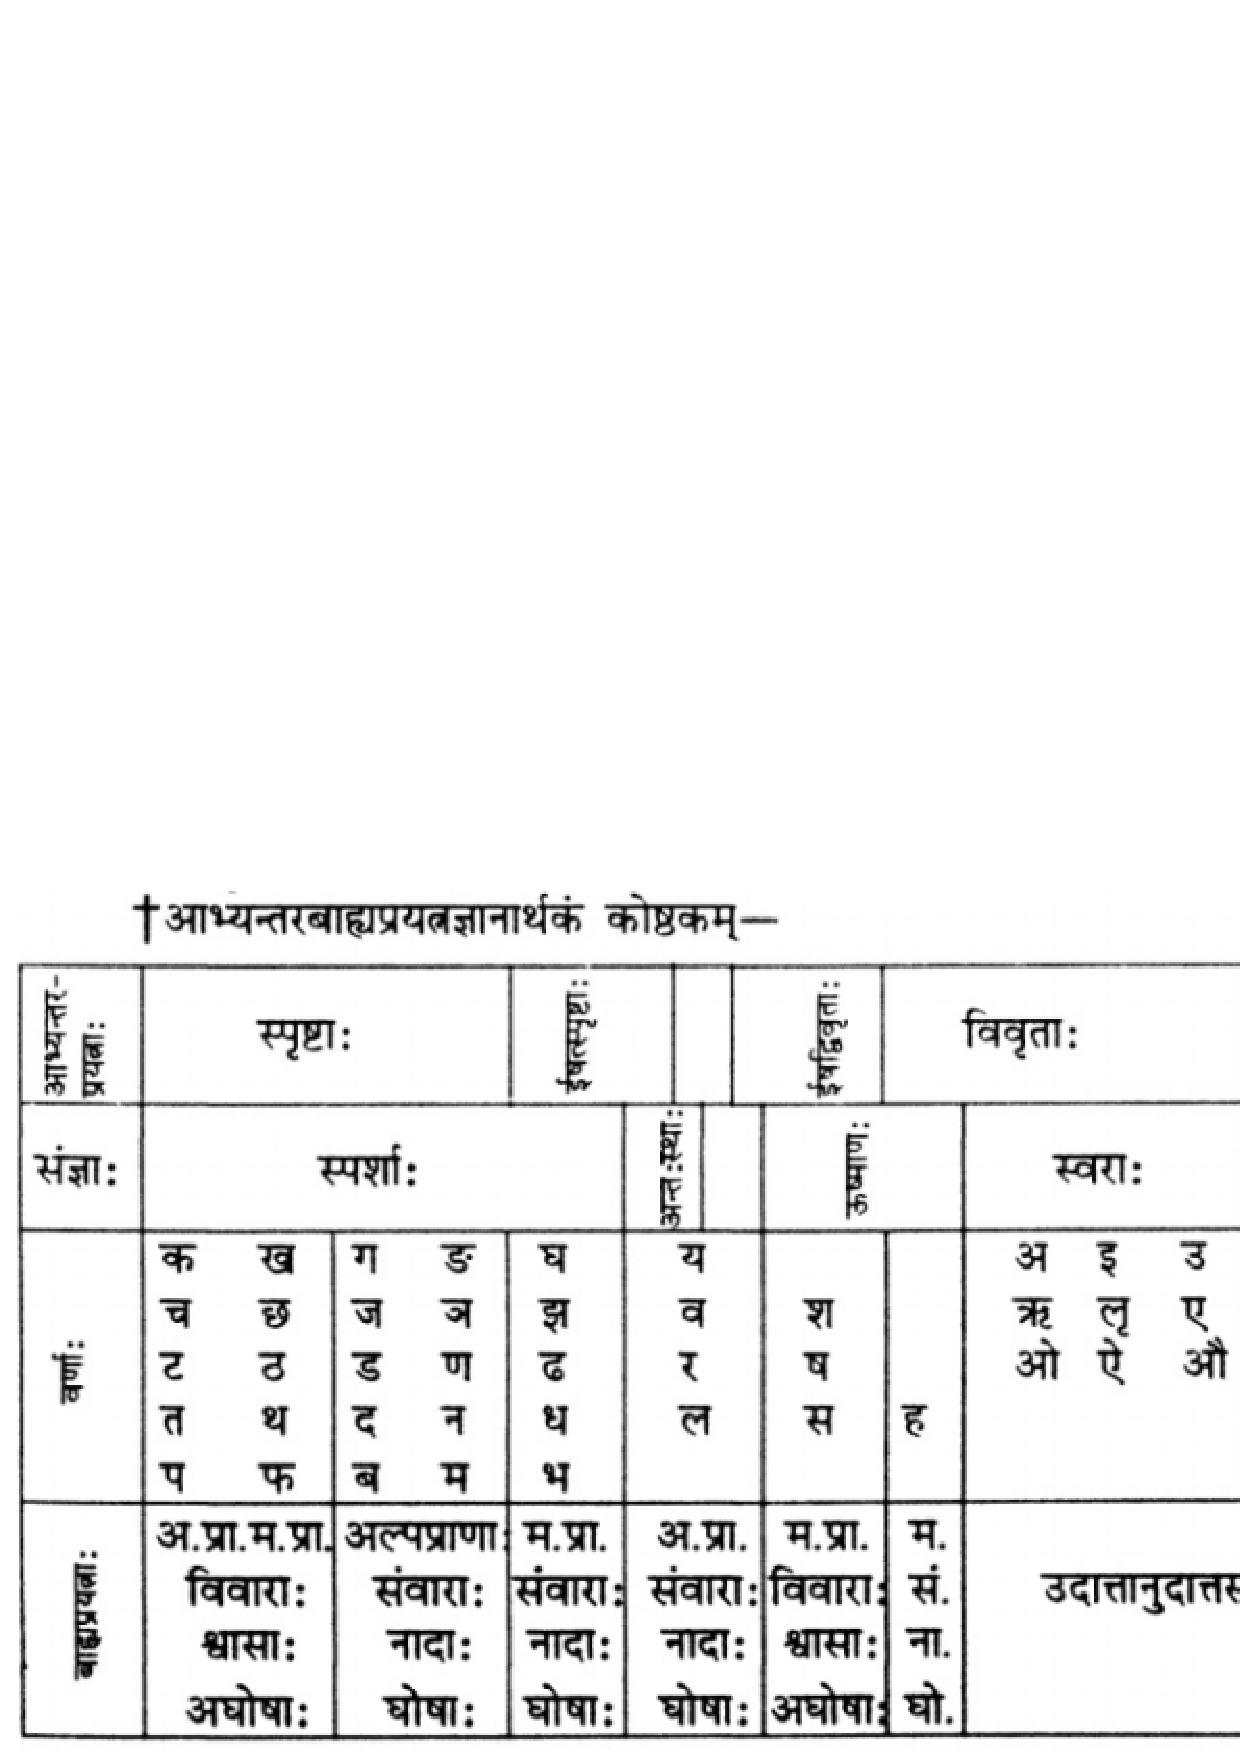
\includegraphics{"images/article-03/art03-fig01.png"}
\end{center}

Where exactly in the Sanskrit native tradition are \dev{अ, इ, उ} called “Vowels” and amongst “Vowels”, “Primary” (as “put briefly” (Bryant 2001:70) in a chapter with an arguably gratuitous subtitle: \textit{The Dethronement of Sanskrit})? \dev{अ, इ, उ} are, as per Sanskrit tradition, without doubt a \textit{mātra} shorter than \dev{ए, ओ} but what native Sanskrit category calls them “Primary” amongst “vowels” and just because \dev{ए, ओ} have a \textit{mātra} more, does that mean one can make a statement that Sanskrit offers “a simple vowel triad (/i,a,u/)” rather than a “PIE array of /i, e, a, o, u/”? More importantly, is the comparison of /i, e, a, o, u/ and \dev{अ, इ, उ, ए, ओ} even a meaningful comparison? Can the fact that Sanskrit’s sophistication in having an internal logic to separate \dev{अ, इ, उ} from \dev{ए, ओ} on counts such as \textit{mātra}\index{matra@\textit{mātra}} (whilst being in the same category native-to-tradition category \textit{svara}) be extrapolated to make the point that “Sanskrit offers “a simple vowel triad (/i.a,u/)” rather than a “PIE array of /i, e, a, o, u/”?

As a response to the second point, the supposed “lack of representation of for short \textit{e} and \textit{o} in the Sanskrit alphabet,” an insider could ask whether the following been considered:

\begin{myquote}
“On going through Patañjali’s commentary on the sutras of Pāṇini, I discovered that Sanskrit too has these short vowels and it was a comforting discovery. Patañjali says that, in chanting the \textit{Satyamugri} and \textit{Ranayaniya} Śākhās of the Sāmaveda the short “e” and “o” are used.” \endnote{Also, see: (P\_1,1.48) KA\_I,117.4-118.4 Ro\_I,357-359 \{38/46\} \textit{nanu ca bhoḥ chandogānām sātyamugrirāṇāyanīyāḥ ardham ekāram ardham okāram ca adhīyate: sujāte eśvasūnṛte, adhvaryo odribhiḥ sutam, śukram te enyat yajatam te enyat iti}}

~\hfill (Sarasvati 2008:295)
\end{myquote}

The idea of refuting the two points above is not to claim Sanskrit as PIE but to simply highlight, what appears to us, to be serious methodological flaws—flawed comparison, flawed reasoning, not rooted in Sanskrit tradition (amongst others)—which are attributed as reasons—not by us, but by linguists themselves—for Sanskrit being relegated to a sister status, rather than the more-or-less exact preserver of the original language. Those who advance either the Out-of-India theory or the theory that Sanskrit is the original PIE might, though, find the above two refutations of some use.

\begin{myquote}
"Any possibility that Sanskrit as a language and the Vedic tradition could have evolved in India remains an anathema in the eyes of the Europeans and the cause of relentless attacks on India.... \textbf{Assertions and claims, even though put forward with unshakable conviction, when looked critically appear to be based on beliefs and assumptions, and not compelling or credible evidence. And yet the same belief based dogmatic assertions remain the guiding principles of the Western mindset, with little response from Indian scholarship to contest, challenge and overturn what in most instances should be easily refutable}."\hfill (Singh 2017:18) [Emphasis ours]
\end{myquote}

While undertaking a detailed review of every Indo-European law with a Sanskrit connection (Table 2 shows at least 17) and instantiating all Western appropriations from Sanskrit would be too vast in scope to be dealt with in any depth here that does justice to these full-fledged independent research topics, like our treatment of one Indo-European law—significant enough for linguists to attribute it to at least five scholars and for relegating “Sanskrit” as a “sister” of Greek and Latin)—and questioning attributions by Goldsmith and Laks to whom they call “the first great American linguist” (Goldsmith \& Laks 2016:89)—William Dwight Whitney—might be a small addition to Professor Subrahmanyam’s catalogue of Western linguistic appropriations and digestion.

\begin{myquote}
In \textit{Language and Mind Sciences} Goldsmith and Laks not only call Whitney “first great American linguist”, but also provide a diagram—Fig. 2.2.(Goldsmith and Laks 2016:93)—which makes clear his nodal role between nine subsequent linguists (including five of the “neogrammarians”) and seven linguists before him. According to Goldsmith and Laks, it was Whitney who “\textbf{introduced the various parts of the articulatory apparatus—the lungs, the larynx, the pharynx, the parts of the mouth}. In short, voice was “the audible result of a column of air emitted by the lungs, impressed with sonancy and variety of pitch by the larynx, and individualized by the mouth-organs.””

~\hfill (Goldsmith \& Laks 2016:96) [Emphasis ours]
\end{myquote}

They then add:

\vskip 2pt

\begin{myquote}
“There were three important positions: \textbf{“one in the front, made by lip against lip, the labial closure, giving p; one in the back of the mouth, made against the soft palate by the rear upper surface of the tongue, the palatal (or guttural) closure, giving k; and one intermediate between the other two, made by the point or front of the tongue against the roof of the mouth near the front teeth, the lingual (or dental) closure, giving t.”} [61-2]. He put this together graphically in a simple chart:”\hfill (Goldsmith \& Laks 2016:96) [Emphasis ours]
\end{myquote}

\vskip 3pt

\begin{myquote}
“All of this sounds quite modern and up to date, but there is more, and \textbf{we wish to emphasize this fact because what he wrote next is often taken to be an insight that was not made explicit until the work of the Prague Circle in the 1930s. “Along with k,t,p, in the first place, go their nearest kindred, g,d,b,” Whitney wrote, and he referred to g as the sonant, or vocal, “counterpart” of k, and so on}.”

~\hfill (Goldsmith \& Laks 2016:97) [Emphasis ours]
\end{myquote}

All three excerpts emphasized above (first and third being unarguably explicit attributions to Whitney), in our view, can be attributed to Pāṇini\index{Panini@Pāṇini} through others in his tradition rather than Whitney. This is easily verified when one considers points 13 to 16 (Ballantyne 1849:4-7) in the English translation titled \textit{The Laghu Kaumudi, A Sanskrit Grammar by Varadaraja} published just about a year before Whitney left for Germany to study Sanskrit.



\section{Conclusions}

In our analysis, we have considered, in section 2 of the paper, some of the recent 2017 evidence from mainstream Western academia and Indian politics and observed how not only the Aryan Migration (into India) Theory, but also its supposedly discredited predecessor Aryan Invasion Theory are privileged in certain textbooks and courses, which hence make an Insider analysis and critique of this seemingly beaten-to-death topic not so redundant. In section 3, bearing in mind future treatments of this topic, we have attempted dimensionalising the problem: firstly, by establishing that western linguistics is not and cannot be the primary source for a resolution of this problem (especially when it relates to the origins of Indian civilization and consequently chronology of ancient India) even if western linguistics were the primary sustainer of this problem for over two centuries; secondly, demonstrating, through a detailed search-list-analyse study of occurrences of \textit{ārya} and \textit{drāviḍa} in some of the earliest indigenous (Sanskrit) texts, no basis for an Aryan Invasion/Migration into India accompanied with import of Sanskrit and Rig Veda, and thirdly, through a step towards a \textit{pūrva-pakśa} of Indo-European linguistics, highlighted differences in positions even within linguists vis-a-vis the robustness of their methods, included some of the critiques of the domain's methods from other academic fields, took a closer look at more recent quantitative studies whose results can be interpreted to weaken some aspects of supposedly established aspects of Indo-Aryan and Dravidian languages, also compiled, in order to facilitate further research, a chronological frame of 88 names (between 1100 CE and 1900 CE), majority of whom are acknowledged in recent mainstream linguistic publications as part of the Indo-European linguistics tradition, and finally examined closely, assumptions of an important Indo-European (so-called) ``law" and attributions to "the first great American linguist." We believe that the combination of the above addresses specific voids in Insider efforts in addressing this problem, even as it brings together arguments from diverse fields and scholars that would advance an Insider position on this matter.

\newpage

As one looks back at the work which lies at the very inception of the outrageous theory of Aryan Invasion/Migration into India, one sees not only the progressive paths traced by science, be it through evolution or the dismissal of the concept of race, but also the role played by one of the most fundamental tools of practising history - comparison. William Jones’s find of the commonalities seen across the languages of Sanskrit, Persian, German, Greek and Latin hinges entirely on this method. At the heart of comparison as \textit{modus operandi}, lies chronology. In purposefully setting up a comparison between the Oriental and Occidental cultures, the colonial Indologists laid the basis for not only studying the resemblances between the two, but also the timelines that formed the backdrops for the respective cultures. In doing so, the wise, prosperous ancient India had to make way for the dullard and poor one to justify Pax Britannica’s rule. Chronology of India thus found itself defaced and vandalised to be boxed in a manner the coloniser chose. It is indeed shocking that native accounts and methods of the pandit were not only mocked at and discarded but also openly replaced with the revised narratives that were constructed on suspect foundations, provided by the European academia and missionaries alike. The casualties that resulted from this blow range from the dating of the \textit{Veda-s} to historical events and literary and other cultural creations. We authors in our previous work have shown in detail the impact of the altered British chronology in dating several of ancient India’s kings, works such as the \textit{Nātyaśāstra}, \textit{Aśtādhyāyi}, and even the very act of introducing writing in India. In a brilliant masterstroke, the British, by altering the very basis of India’s history—her chronology—reduced her to a people that desperately sought delusional ideas of antiquity on one hand to believing the coloniser’s falsehoods and falling prey to divisive forces amidst her own. The debate between the \textit{ārya}\index{arya@ārya} and \textit{drāviḍa}\index{dravida@drāviḍa} forces seen to this day, be it in political or social spheres, is a prime example of the latter. Thus, by reordering the chronology of the land, the oppressor equipped himself with tools to desacralise its most cherished and formative aspects, even as he appropriated that which could strengthen his own cultural assets or create new ones disconnected from its source.


\section*{Bibliography}

\begin{thebibliography}{99}
\bibitem{chap3-key01} Ambedkar, B.R. (1947). \textit{Who Were The Shudras?} Bombay: Thacker and Co.

 \bibitem{chap3-key02} Ballantyne, James R. (1849). \textit{The Laghu Kaumudi: A Sanskrit Grammar by Varadaraja with an English Version, Commentary, and Reference}. Benaras: Medical Hall Press, London:Turner\& Co. 

 \bibitem{chap3-key03} Bendall, Herbert (1874). \textit{A compendium of the Comparative Grammar of the Indo-European, Sanskrit, Greek and Latin languages by August Schleicher} translated from the third german edition Part 1. London: Trübner \& Co., 57 and 59, Ludgate Hill. 

 \bibitem{chap3-key04} Benware, Wilbur A. (1974). \textit{The Study of Indo-European Vocalism in the 19\supskpt{th} century: From the Beginnings to Whitney \& Scherer.} Amsterdam/ Philadelphia: John Benjamins Publishing Company 

 \bibitem{chap3-key05} Bod, Rens (2013). \textit{A New History of the Humanities: The Search for Principles and Patterns from Antiquity to Present}. Oxford University Press

 \bibitem{chap3-key06} Borin, Lars; Saxena, Anju; Rama, Taraka; Comrie, Bernard (2014). \textit{Linguistic landscaping of South Asia using digital language resources: Genetic vs. areal linguistics}, LREC Conferences 20

 \bibitem{chap3-key07} Bryant, Edwin (2001). \textit{The Quest for the Origins of Vedic Culture The Indo-Aryan Migration Debate}. New York: Oxford University Press Inc

 \bibitem{chap3-key08} Campbell, Lyle (1998). \textit{Historical Linguistics An Introduction}. First MIT Press edition, 1999. Originally published in 1998 by Edinburgh University

 \bibitem{chap3-key09} Campbell, Lyle and Poser, William J. (2008). \textit{Language Classification History and Method}. Cambridge University Press

 \bibitem{chap3-key10} Clackson, James (2007). \textit{Indo-European Linguistics An Introduction}. Cambridge University Press

 \bibitem{chap3-key11} Clackson, James (2013). \textit{The Origin of the Indic Languages – The Indo-European Model}, in \textit{Perspectives on the Origin of Indian Civilization} (ed. Marcantonio, Angela and Jha, Girish Nath), Dartmouth: Center for Indic Studies, University of Massachusetts and New Delhi: D.K. Printworld (P) Ltd.

 \bibitem{chap3-key12} Collinge, N.E. (1985). \textit{The laws of Indo-European}. Amsterdam/Philadelphia: John Benjamins Publishing

 \bibitem{chap3-key13} Danino, Michel (2016; Revised August 2017). \textit{The Aryan Issue.} Academia: \url{https://www.academia.edu/30375915/The_Aryan_Issue_-_Michel_Danino}

 \bibitem{chap3-key14} Demoule, Jean-Paul (2016). \textit{The canonical Indo-European model and its underlying assumptions}, FAITS DE LANGUES Comparatisme et reconstruction: tendances actuelles

 \bibitem{chap3-key15} Doniger O’Flaherty, Wendy (1981). \textit{The Rig Veda An Anthology}. London/NY/Toronto/Dublin/New Delhi/Australia/New Zealand/South Africa: Penguin group

 \bibitem{chap3-key16} Elst, Koenraad (2013). \textit{Some unlikely tentacles of Early Indo-European, }in \textit{Perspectives on the Origin of Indian Civilization }(ed. Marcantonio, Angela and Jha, Girish Nath). Dartmouth: Center for Indic Studies, University of Massachusetts and New Delhi: D.K. Printworld (P) Ltd.

 \bibitem{chap3-key17} Goldsmith, John and Laks, Bernard (2016). \textit{Language and Mind Sciences The First Four Generations}, Part II – \textit{The 19\supskpt{th} century and language}

 \bibitem{chap3-key18} Heggarty, Paul (2014). \textit{Prehistory through language and archaeology from: The Routledge Handbook of Historical Linguistics Routledge} Editors - Bowern, Claire and Evans, Bethwyn 

 \bibitem{chap3-key19} Hopkins, Edward W (1883). \textit{Words for Color in the Rig Veda}. The American Journal of Philology, Vol. 4, No. 2

 \bibitem{chap3-key20} Hubey, H.M. (2002). \textit{Logic, Fallacy, Reasoning and Superficial Resemblance}, \url{https://www.montclair.edu/profilepages/media/344/user/logicfallacyreasoningandsuperficial.pdf}

 \bibitem{chap3-key21} Jamison, Stephanie (2006). JIES REVIEWS \#3 – Culture (pp 255–261), The Journal of Indo-European Studies, Volume 34, Number 1 \& 2, Spring/Summer 2006

 \bibitem{chap3-key22} Jha, Girish Nath (2013). \textit{Some remarks on the Origin and Development of Indian Languages and Linguistic Area,} in \textit{Perspectives on the Origin of Indian Civilization} (ed. Marcantonio, Angela and Jha, Girish Nath). Dartmouth: Center for Indic Studies, University of Massachusetts and New Delhi: D.K. Printworld (P) Ltd

 \bibitem{chap3-key23} Keppens, Marianne \& Roover, J.(2014). \textit{Orientalism and the Puzzle of the Aryan Invasion Theory}. Pragmata: Journal of Human Sciences 2,2\break 51–76

 \bibitem{chap3-key24} Lehmann, W.P. (1967). \textit{A Reader in Nineteenth Century Historical Indo-European Linguistics. } Bloomington: Indian University Press

 \bibitem{chap3-key25} Malhotra, Rajiv and Neelakandan, Aravindan (2011). \textit{Breaking India: Western Interventions in Dravidian and Dalit Faultlines}. New Delhi: AMARYLLIS An Imprint of Manjul Publishing House Pvt. Ltd.

 \bibitem{chap3-key26} Marcantonio, Angela (2013). \textit{Perspectives on the Origin of Indian Civilization}, in \textit{Perspectives on the Origin of Indian Civilization} (ed. Marcantonio, Angela and Jha, Girish Nath), Dartmouth: Center for Indic Studies, University of Massachusetts and New Delhi: D.K. Printworld (P) Ltd

 \bibitem{chap3-key27} Pereltsvaig, Asya and Lewis, Martin W. (2015). \textit{The Indo-European Controversy Facts and Fallacies in Historical Linguistics}, Cambridge University Press

 \bibitem{chap3-key28} Petersen, Wiebke (2009). \textit{On the Construction of Sivasutra-Alphabets}. \url{https://user.phil.hhu.de/~petersen/paper/Petersen_SanskritSymp2009.pdf}

 \bibitem{chap3-key29} Poliakov, Leon (1971). \textit{The Aryan Myth.} Paris: Calmann Levy

 \bibitem{chap3-key30} Prasanna, T.R.S. (2012). “\textit{There is no scientific basis for the Aryan Invasion Theory”}. Current Science, Vol. 103, No. 2

 \bibitem{chap3-key31} Proceedings of the Paris Anthropological Society, The Anthropological Review, Vol. 5, No. 18/19 (Jul. - Oct., 1867), Published by: Royal Anthropological Institute of Great Britain and Ireland

 \bibitem{chap3-key32} Renfrew, Colin (2017). \textit{Enduring conundrum – Indo-European relationships} in \textit{European Archaeology Identities And Migrations.} Ed. Manolakakis, Laurence et. al. Leiden:Sidestone Press

 \bibitem{chap3-key33} Rocher, Rosane In Koerner, R.F.K and Asher, R.E., Ed. (1995). \textit{Discovery of Sanskrit by Europeans, }in \textit{Concise History of the Language Sciences: From the Sumerians to Cognitivists.}, PERGAMON, Cambridge University Press

 \bibitem{chap3-key34} Sarasvati, Candrasekharendra (2008). \textit{Hindu Dharma}. Mumbai: Bhavan’s Book University 

 \bibitem{chap3-key35} Sengupta, Debapriya and Saha, Goutam (2015). \textit{Study on Similarity among Indian Languages Using Language Verification Framework}. Advances in Artificial Intelligence, Volume 2015 (2015), Article ID 325703

 \bibitem{chap3-key36} Shaffer, Jim G. and Lichtenstein, Diane A. (2013). \textit{South Asian Archaeology}, in Perspectives \textit{on the Origin of Indian Civilization} (ed. Marcantonio, Angela and Jha, Girish Nath). Dartmouth: Center for Indic Studies, University of Massachusetts and New Delhi: D.K. Printworld (P) Ltd

 \bibitem{chap3-key37} Singh, Varun(2017). \textit{Origin of Hindu Religion and Sanskrit in Central Asia: A Recent Claim and Its Rebuttal}. Indian Historical Review 44(1) 1–20

 \bibitem{chap3-key38} Sri Aurobindo, (1998). \textit{The Secret of The Veda}. \textit{Volume 15, The Complete Works Of Sri Aurobindo.} Pondicherry: Sri Aurobindo Ashram Publication Department

 \bibitem{chap3-key39} Staal, Fritz (1972). \textit{A Reader on the Sanskrit Grammarians}. Massachusetts Institute of Technology

 \bibitem{chap3-key40} Subrahmanyam, Korada (2008). \textit{Theories of Language Oriental and Occidental}. New Delhi: D.K. Printworld (P) Ltd. 

 \bibitem{chap3-key41} Thomas, Margaret (2011). \textit{Fifty Key Thinkers on Language and Linguistics}. Oxon:Routledge

 \bibitem{chap3-key42} Tod, James (1957). \textit{Annals and Antiquities of Rajasthan}. 2 vols London: Routledge and Kegan Paul

 \bibitem{chap3-key43} Trautmann, Thomas R. (2007). \textit{The Aryan Debate.} New Delhi\textit{: }Oxford University Press

 \bibitem{chap3-key44} Witzel, Michael (2001). “\textit{Autochthonous Aryans? The evidence from Old Indian and Iranian Texts”}. Electronic Journal of Vedic Studies 7–3 (EJVS) 2001 (1–115)

 \end{thebibliography}

\theendnotes

